\chapter{光谱与结构}\label{ch:b1:structure-spectroscopy}

一位调香师交给实验室一瓶无色液体，闻起来有菠萝香味，
并问这是什么。五十年前，
要回答这个问题需要数周的降解反应。如今只需十分钟：元素分析给出化学式，
红外光谱确定官能团，质子核磁共振谱显示原子之间的连接方式。
本章讲解如何读取每一种光谱，
说明不同波段的光对分子有何作用，
以及光谱中哪些特征对应哪一部分结构，
最后以这个
菠萝分子作结。

\begin{recall}
学校分册（十一、十二年级）用分光光度计测量\omterm{def:b1:structure-spectroscopy:absorbance}{吸光度}，
利用比尔–朗伯定律求浓度，
依据红外吸收谱带表识别官能团，并读取简单的质子核磁共振谱，
包括峰的数目、\omterm{def:b1:structure-spectroscopy:integration}{积分}面积以及 $n + 1$ 规则。
单键、双键、三键以及 $\pi$ 键，
见\cref{ch:b1:lewis-resonance-vsepr}。
\end{recall}

\section{紫外–可见光谱：共轭与颜色}

\begin{definition}[吸光度与比尔–朗伯定律]\label{def:b1:structure-spectroscopy:absorbance}
设强度为 $I_0$ 的光射入溶液，
射出时强度为 $I$，称 $A = \log(I_0/I)$ 为\emph{吸光度}\index{吸光度}。
对于只含一种吸光物质的稀溶液，有 $A = \varepsilon\,\ell\,c$
（比尔–朗伯定律），
其中 $\ell$ 为光程，$c$ 为浓度，
$\varepsilon$ 为\emph{摩尔吸光系数}\index{摩尔吸光系数}，
是该物质在该波长下的性质。
\end{definition}

当光子能量与分子化学键中被占据的最高\omterm{def:b1:quantum-numbers:energy-level}{能级}
和最低空\omterm{def:b1:quantum-numbers:energy-level}{能级}之间的能隙相等时，分子吸收紫外光或可见光。
$\sigma$ 键的能隙很大，吸收位于远紫外区；
$\pi$ 键的吸收更接近可见光区，
由双键与单键交替构成的链，
链越长，吸收波长越长。

\begin{definition}[共轭体系、发色团、最大吸收波长]\label{def:b1:structure-spectroscopy:conjugation}
\emph{共轭体系}\index{共轭体系}是由原子组成的链，
其中每个原子都带有一个 $p$ 轨道，并处于 $\pi$ 体系中，
如双键与单键交替排列（1,3-丁二烯、苯）。引起某一吸收的原子团
称为其\emph{发色团}\index{发色团}；
\omterm{def:b1:structure-spectroscopy:absorbance}{吸光度}最大时所对应的波长
称为\emph{最大吸收波长}\index{最大吸收波长}，记作 $\lambda_{\max}$。
\end{definition}

\omterm{def:b1:structure-spectroscopy:conjugation}{共轭体系}的\omterm{def:b1:quantum-numbers:energy-level}{能级}分布于整条链上，
并随链的增长而彼此靠近，这与一维长箱中粒子的\omterm{def:b1:quantum-numbers:energy-level}{能级}变化相同，
$\lambda_{\max}$ 随共轭程度增大而增大。
乙烯和丁二烯只在紫外区吸收；
$\beta$-胡萝卜素中的十一个共轭双键使吸收移至可见光的蓝色部分。
物质所呈现的颜色与其所吸收的光互补，
吸收蓝色和紫色光的胡萝卜素呈橙色。

\begin{omfigure}
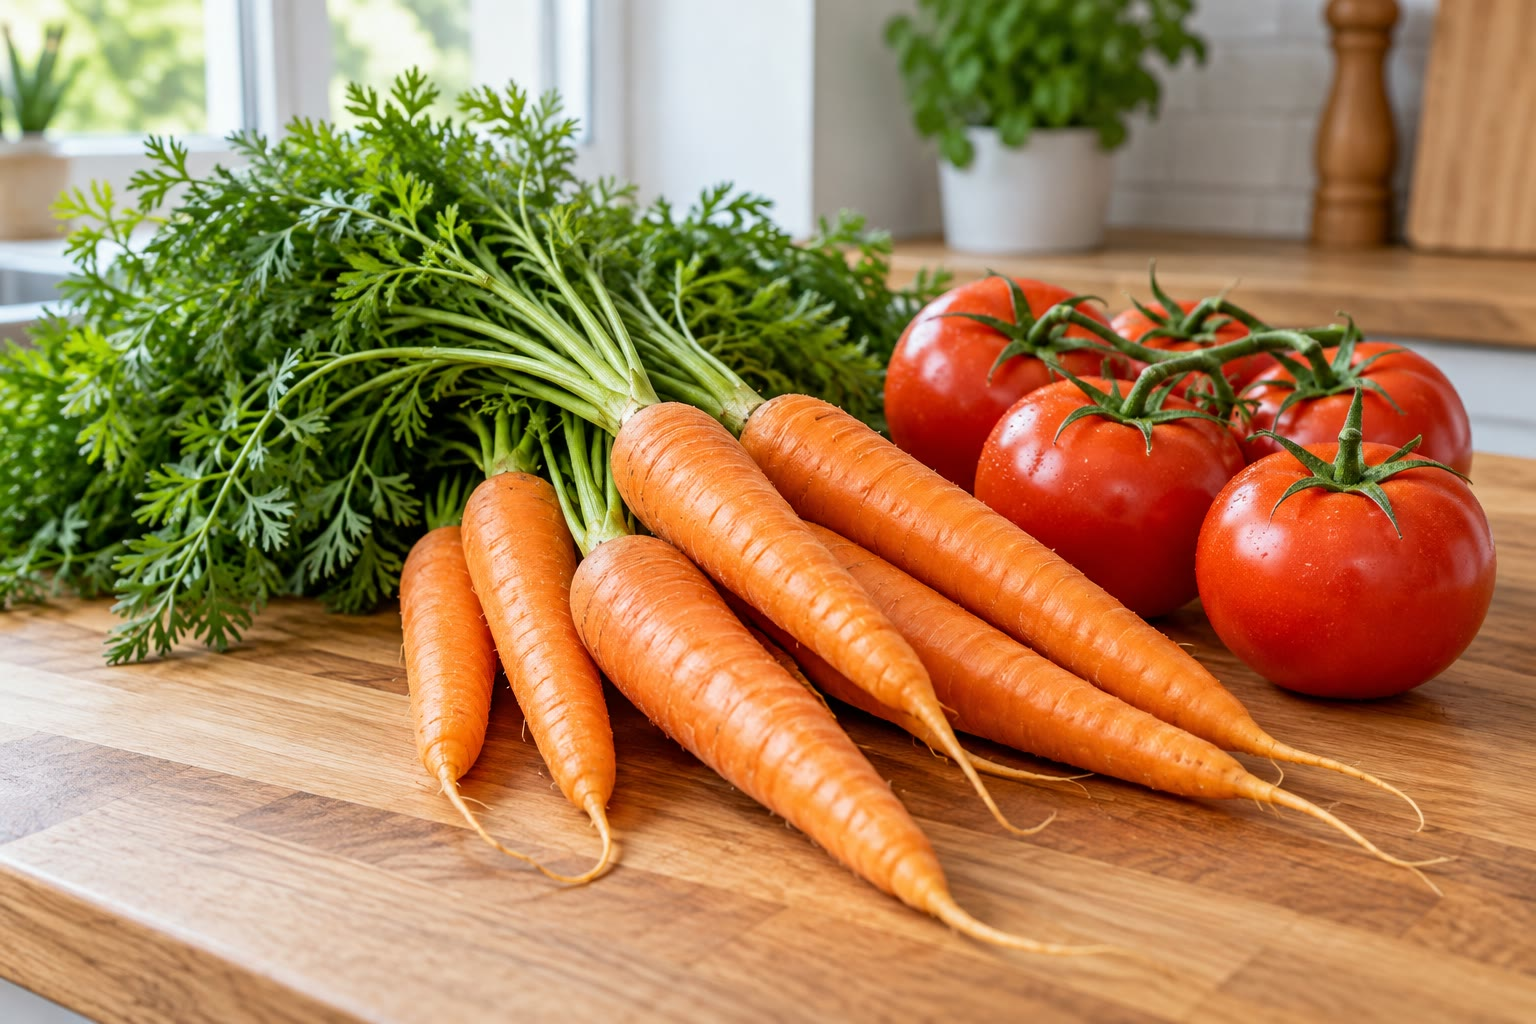
\includegraphics[width=0.55\linewidth]{images/book2/ai/b1-17-carrots-tomatoes.jpg}

{\small 胡萝卜和番茄的颜色源于长链共轭分子，
即胡萝卜素和番茄红素，它们吸收蓝光和绿光，
让橙光和红光透过。}
\end{omfigure}

\begin{omfigure}
\begin{tikzpicture}[font=\small]
  \foreach \a/\c/\n in {90/red/红, 30/orange/橙, -30/yellow/黄, -90/green!70!black/绿, -150/blue/蓝, 150/violet/紫} {
    \fill[\c] (0,0) -- (\a-30:1.4) arc[start angle=\a-30, end angle=\a+30, radius=1.4] -- cycle;
    \node at (\a:1.85) {\n};
  }
  \draw[<->, thick] (-150:0.9) -- (30:0.9);
  \node[align=left, anchor=west] at (2.6,0.3) {吸收蓝色 $\Rightarrow$ 呈橙色 \\（互补色在色轮上彼此相对）};
\end{tikzpicture}

{\small 色轮。所见颜色是所吸收颜色的补色，
吸收蓝色的溶液呈橙色。}
\end{omfigure}

\section{红外光谱深入}

\begin{definition}[波数、透射比、指纹区]\label{def:b1:structure-spectroscopy:wavenumber}
红外光谱以\emph{波数}\index{波数}为横坐标作图，
$\tilde\nu = 1/\lambda$，单位为 \unit{cm^{-1}}，与光子能量成正比。
纵坐标为\emph{透射比}\index{透射比} $T = I/I_0$，以百分数表示，
因此吸收峰向下。在约
\qty{1500}{cm^{-1}} 以下，许多相互重叠的谱带
反映的是整个分子而非某一个化学键的特征，它们构成
\emph{指纹区}\index{指纹区}。
\end{definition}

化学键在其振动频率处吸收红外光。
如同两个质量由弹簧相连，
化学键越强、原子越轻，\omterm{def:b1:structure-spectroscopy:wavenumber}{波数}越高：
与氢相连的键（O--H、C--H）位于 \qty{2800}{cm^{-1}} 以上，
三键在 2200 附近，双键在 1700--1600 附近，
较重原子间的单键在 1300 以下。下表给出本章分子在气相中的实测位置，
气相中分子彼此孤立。

\begin{omfigure}
\begin{tabular}{llr}
\hline
分子 & 化学键 & $\tilde\nu$ (\unit{cm^{-1}}) \\
\hline
乙醇 & O--H & 3666 \\
乙醇 & C--H & 2978 \\
乙醇 & C--O & 1060 \\
丙酮 & C=O & 1738 \\
乙酸 & O--H & 3582 \\
乙酸 & C=O & 1788 \\
乙酸乙酯 & C=O & 1764 \\
乙酸乙酯 & C--O & 1238 \\
\hline
\end{tabular}

\smallskip
{\small 气相红外光谱中的吸收峰位置。在液体中，\omterm{def:b1:intermolecular-forces-solvents:hbond}{氢键}
使 O--H 峰变宽并移向较低\omterm{def:b1:structure-spectroscopy:wavenumber}{波数}，而
酸的 C=O 峰随酸分子缔合而下移。}
% ledger: ir:ethanol-OH, ir:ethanol-CH, ir:ethanol-CO, ir:propanone-CO, ir:ethanoic-OH, ir:ethanoic-CO, ir:ethylethanoate-CO, ir:ethylethanoate-COC
\end{omfigure}

\begin{omfigure}
\begin{tikzpicture}
\begin{axis}[name=i1, width=0.86\linewidth, height=3.2cm, xmin=500, xmax=4000, x dir=reverse, ymin=0, ymax=105, ytick={0,50,100}, ylabel={$T$ (\%)}, tick label style={font=\scriptsize}, label style={font=\small}, xticklabels={}]
\addplot[omDef, thick] table[x=nu, y=T] {figdata/out/bachelor-1-spectra-ir-ethanol.dat};
\node[font=\scriptsize, anchor=west] at (axis cs:2600,25) {乙醇};
\end{axis}
\begin{axis}[name=i2, at={(i1.south)}, anchor=north, yshift=-0.25cm, width=0.86\linewidth, height=3.2cm, xmin=500, xmax=4000, x dir=reverse, ymin=0, ymax=105, ytick={0,50,100}, ylabel={$T$ (\%)}, tick label style={font=\scriptsize}, label style={font=\small}, xticklabels={}]
\addplot[omProp, thick] table[x=nu, y=T] {figdata/out/bachelor-1-spectra-ir-propanone.dat};
\node[font=\scriptsize, anchor=west] at (axis cs:2600,25) {丙酮};
\end{axis}
\begin{axis}[at={(i2.south)}, anchor=north, yshift=-0.25cm, width=0.86\linewidth, height=3.2cm, xmin=500, xmax=4000, x dir=reverse, ymin=0, ymax=105, ytick={0,50,100}, ylabel={$T$ (\%)}, tick label style={font=\scriptsize}, label style={font=\small}, xlabel={波数 (\unit{cm^{-1}})}]
\addplot[omMeth, thick] table[x=nu, y=T] {figdata/out/bachelor-1-spectra-ir-ethanoic.dat};
\node[font=\scriptsize, anchor=west] at (axis cs:2600,25) {乙酸};
\end{axis}
\end{tikzpicture}

{\small 乙醇、丙酮和乙酸的红外光谱，
由表中测得的吸收峰位置模拟得到
（峰高与峰宽为示意）。约 \qty{1750}{cm^{-1}} 处的 C=O 峰与
高于 \qty{3500}{cm^{-1}} 的 O--H 峰，可
一眼区分这三类官能团。}
\end{omfigure}

\section{质子核磁共振：化学位移与积分}

在强磁场中，质子具有两个\omterm{def:b1:quantum-numbers:energy-level}{能级}；频率恰当的无线电波
可使质子在两\omterm{def:b1:quantum-numbers:energy-level}{能级}之间跃迁。该频率
正比于质子实际感受到的磁场，而质子周围的电子
会使这一磁场略有削弱。因此，处于不同化学环境中的质子
其共振频率略有不同。

\begin{definition}[化学位移、屏蔽、等价质子]\label{def:b1:structure-spectroscopy:chemical-shift}
质子的\emph{化学位移}\index{化学位移}为
$\delta = (\nu - \nu_{\text{参比}})/\nu_0 \times 10^6$，单位为 \unit{ppm}，其中
$\nu$ 为该质子的共振频率，$\nu_{\text{参比}}$ 为四甲基硅烷中
质子的共振频率，$\nu_0$ 为谱仪的工作频率。电子对原子核处
磁场的削弱称为其
\emph{屏蔽}\index{屏蔽}：吸电子的邻近基团（O、卤素、C=O）
使质子去屏蔽，并使其 $\delta$ 增大。
\emph{等价质子}\index{等价质子}是指通过分子的对称性或快速旋转
而相互交换的质子，它们
具有相同的化学位移。
\end{definition}

\begin{proposition}[化学位移与谱仪无关]\label{prop:b1:structure-spectroscopy:shift-field-independent}
质子的\omterm{def:b1:structure-spectroscopy:chemical-shift}{化学位移}在不同场强的
谱仪上相同。
\end{proposition}

\begin{proof}
$\nu$ 与 $\nu_{\text{参比}}$ 均正比于外加
磁场 $B_0$（各自乘以其\omterm{def:b1:structure-spectroscopy:chemical-shift}{屏蔽}因子），$\nu_0$ 亦然。
因此比值 $(\nu - \nu_{\text{参比}})/\nu_0$ 与
$B_0$ 无关。相反，以赫兹计的差值随场强增大而增大。
\end{proof}

\begin{definition}[积分]\label{def:b1:structure-spectroscopy:integration}
信号的\emph{积分}\index{积分}即其面积，
在谱图上读作阶梯曲线的台阶高度；面积与
产生该信号的质子数成正比。
\end{definition}

\section{自旋–自旋耦合}

\begin{definition}[自旋–自旋耦合、耦合常数、多重峰]\label{def:b1:structure-spectroscopy:coupling}
通过化学键，质子的磁状态会使
相邻碳原子上质子所感受到的磁场略有改变：这种
\emph{自旋–自旋耦合}\index{自旋–自旋耦合}使每个信号分裂为
一组\emph{多重峰}\index{多重峰}，各谱线之间相隔
\emph{耦合常数}\index{耦合常数} $J$，以赫兹计。彼此耦合的两个质子
具有相同的 $J$；\omterm{def:b1:structure-spectroscopy:chemical-shift}{等价质子}
之间不会使对方的信号发生分裂。
\end{definition}

\begin{proposition}[\texorpdfstring{$n + 1$}{n + 1} 规则]\label{prop:b1:structure-spectroscopy:n-plus-one}
一个质子（或一组\omterm{def:b1:structure-spectroscopy:chemical-shift}{等价质子}）以相同的 $J$ 与
$n$ 个等价邻居耦合，则给出 $n + 1$ 条谱线，相邻谱线相隔 $J$，相对强度为
二项式系数 $\binom{n}{k}$，$k = 0$ 至
$n$（即\emph{$n + 1$ 规则}\index{$n + 1$ 规则}）。
\end{proposition}

\begin{proof}
每个邻居处于两种自旋态之一，使观测谱线
移动 $+J/2$ 或 $-J/2$。若有 $n$ 个邻居，则位移为 $(k - n/2)J$，其中 $k$
为处于第一种状态的邻居数：共 $n + 1$ 个值，彼此以 $J$ 等间距排列。
由于两种状态的布居几乎相等，所有 $2^n$ 种组合
等可能出现，而其中 $k$ 个处于第一种状态的组合
共有 $\binom{n}{k}$ 种。
\end{proof}

\begin{omfigure}
\begin{tikzpicture}[font=\small, x=0.85cm, y=0.5cm]
  % quartet: three neighbours, each split +-J/2 (J = 1.5 units)
  \draw[thick] (0,4) -- (0,3.4);
  \foreach \x in {-0.75,0.75} \draw (0,3.4) -- (\x,2.4);
  \foreach \a/\b in {-0.75/-1.5, -0.75/0, 0.75/0, 0.75/1.5} \draw (\a,2.4) -- (\b,1.4);
  \foreach \a/\b in {-1.5/-2.25, -1.5/-0.75, 0/-0.75, 0/0.75, 1.5/0.75, 1.5/2.25} \draw (\a,1.4) -- (\b,0.4);
  \foreach \x/\h in {-2.25/1, -0.75/3, 0.75/3, 2.25/1} {\draw[omDef, very thick] (\x,-2.6) -- (\x,{-2.6+0.7*\h}); \draw[dotted] (\x,0.4) -- (\x,{-2.6+0.7*\h});}
  \draw (-2.8,-2.6) -- (2.8,-2.6);
  \node at (0,-3.4) {四重峰 1\,:\,3\,:\,3\,:\,1 （\ce{-CH2-} 与 \ce{-CH3} 相邻）};
  % triplet: two neighbours
  \begin{scope}[xshift=7.5cm]
  \draw[thick] (0,4) -- (0,3.4);
  \foreach \x in {-0.75,0.75} \draw (0,3.4) -- (\x,2.4);
  \foreach \a/\b in {-0.75/-1.5, -0.75/0, 0.75/0, 0.75/1.5} \draw (\a,2.4) -- (\b,1.4);
  \foreach \x/\h in {-1.5/1, 0/2, 1.5/1} {\draw[omProp, very thick] (\x,-2.6) -- (\x,{-2.6+0.7*\h}); \draw[dotted] (\x,1.4) -- (\x,{-2.6+0.7*\h});}
  \draw (-2.1,-2.6) -- (2.1,-2.6);
  \draw[<->] (-1.5,-0.6) -- (0,-0.6) node[midway, above, font=\scriptsize] {$J$};
  \node at (0,-3.4) {三重峰 1\,:\,2\,:\,1 （\ce{-CH3} 与 \ce{-CH2-} 相邻）};
  \end{scope}
\end{tikzpicture}

{\small 分裂树。每个邻近核使每条谱线一分为二，间距为 $J$
；重合谱线的强度相加，得二项式强度。}
\end{omfigure}

\begin{omfigure}
\begin{tikzpicture}
\begin{axis}[name=ea,
  width=0.86\linewidth, height=4.2cm, xmin=0.8, xmax=4.5, x dir=reverse, ymin=0, ymax=1.15,
  axis x line=bottom, axis y line=none, xlabel={化学位移 $\delta$（ppm）},
  tick label style={font=\scriptsize}, label style={font=\small}]
\addplot[omDef, thin] table[x=ppm, y=I] {figdata/out/bachelor-1-spectra-nmr-ethylethanoate.dat};
\node[font=\scriptsize, anchor=south] at (axis cs:4.12,0.75) {四重峰，2H};
\node[font=\scriptsize, anchor=west] at (axis cs:2.0,0.95) {单峰，3H};
\node[font=\scriptsize, anchor=west] at (axis cs:1.15,0.8) {三重峰，3H};
\node[font=\small, anchor=north] at (axis cs:3.0,1.1) {\ce{CH3COOCH2CH3}};
\end{axis}
\begin{axis}[at={(ea.south)}, anchor=north, yshift=-1.3cm,
  width=0.86\linewidth, height=4.2cm, xmin=0.8, xmax=4.5, x dir=reverse, ymin=0, ymax=1.15,
  axis x line=bottom, axis y line=none, xlabel={化学位移 $\delta$（ppm）},
  tick label style={font=\scriptsize}, label style={font=\small}]
\addplot[omProp, thin] table[x=ppm, y=I] {figdata/out/bachelor-1-spectra-nmr-ethanol.dat};
\node[font=\scriptsize, anchor=south] at (axis cs:3.69,0.75) {四重峰，2H};
\node[font=\scriptsize, anchor=west] at (axis cs:2.55,0.6) {单峰，1H};
\node[font=\scriptsize, anchor=west] at (axis cs:1.1,0.8) {三重峰，3H};
\node[font=\small, anchor=north] at (axis cs:2.9,1.1) {\ce{CH3CH2OH}};
\end{axis}
\end{tikzpicture}

{\small 乙酸乙酯（上）与乙醇（下）的质子核磁共振谱，
在 \ce{CDCl3} 中，依据实测\omterm{def:b1:structure-spectroscopy:chemical-shift}{化学位移}与
\omterm{def:b1:structure-spectroscopy:coupling}{耦合常数}模拟 \qty{90}{MHz} 下的谱图（$J = \qty{7.2}{Hz}$ 和 \qty{7.0}{Hz}）。
\ce{OCH2} 的四重峰受氧的去\omterm{def:b1:structure-spectroscopy:chemical-shift}{屏蔽}作用；在乙醇中，OH 质子
在分子间快速交换，不发生耦合，其\omterm{def:b1:structure-spectroscopy:chemical-shift}{化学位移}
随浓度而变。}
% ledger: nmr:ethylethanoate-OCH2, nmr:ethylethanoate-COCH3, nmr:ethylethanoate-CH3, nmr:ethylethanoate-J, nmr:ethanol-CH2, nmr:ethanol-CH3, nmr:ethanol-OH, nmr:ethanol-J
\end{omfigure}

\begin{omfigure}
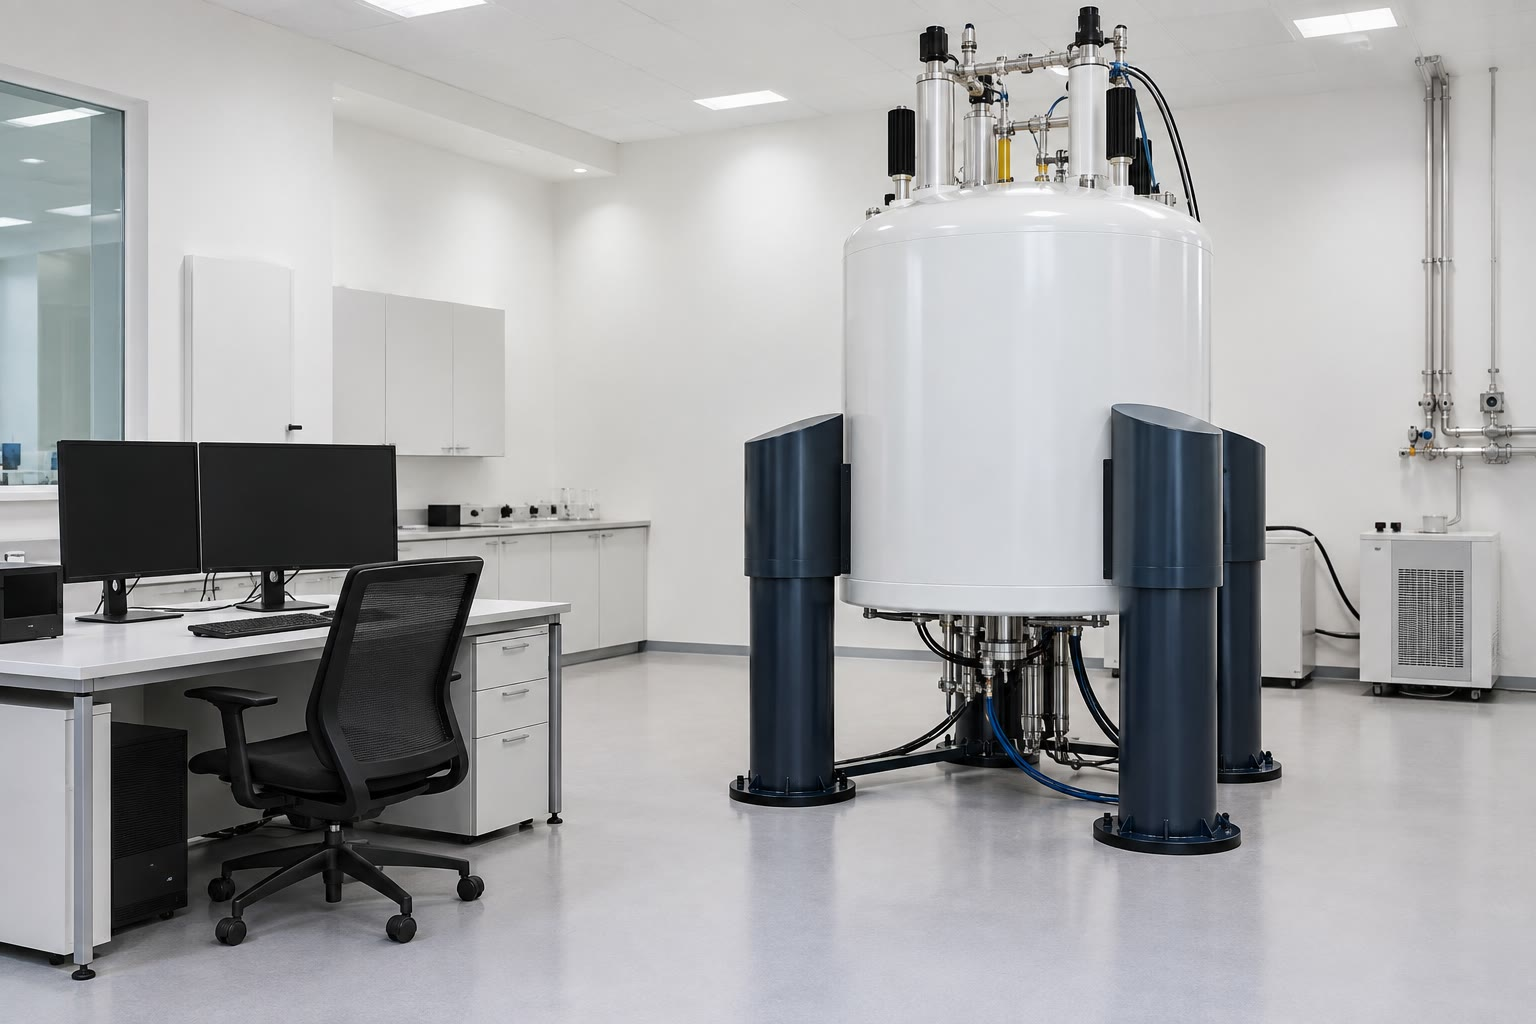
\includegraphics[width=0.5\linewidth]{images/book2/ai/b1-17-nmr.jpg}

{\small 核磁共振谱仪：高大的圆筒内装有一块由液氦冷却的超导
磁铁，样品管被放入其
中心。}
\end{omfigure}

\section{结构推断}

\begin{definition}[不饱和度]\label{def:b1:structure-spectroscopy:unsaturation}
称某分子式的\emph{不饱和度}\index{不饱和度}为
其对应分子中环的个数与 $\pi$ 键
个数之和。
\end{definition}

\begin{proposition}[由分子式求不饱和度]\label{prop:b1:structure-spectroscopy:unsaturation-formula}
对分子 $\mathrm{C}_c\mathrm{H}_h\mathrm{N}_n\mathrm{O}_o\mathrm{X}_x$
（X 为卤素），其\omterm{def:b1:structure-spectroscopy:unsaturation}{不饱和度}为
\[
  D = \frac{2c + 2 + n - h - x}{2} .
\]
\end{proposition}

\begin{proof}
仅含单键、含 $c$ 个碳的开链分子含有 $2c + 2$
个氢原子。每个环或 $\pi$ 键减少两个氢。二价氧
插入链中不改变氢数；三价氮多带一个
氢；卤素取代一个氢。统计缺少的
氢原子数并除以二，即得 $D$。
\end{proof}

\begin{method}[结构推断]\label{met:b1:structure-spectroscopy:solve-structure}
\begin{enumerate}
  \item 由分子式计算 $D$。
  \item 由红外光谱确定官能团（C=O、O--H、N--H、
        C--O），并确认不存在其他官能团。
  \item 由核磁共振谱读取：信号数（等效质子组）、
        \omterm{def:b1:structure-spectroscopy:integration}{积分}（每组质子数）、\omterm{def:b1:structure-spectroscopy:chemical-shift}{化学位移}（邻近基团）、
        多重度（依 $n + 1$ 规则由邻近质子数推得）、
        \omterm{def:b1:structure-spectroscopy:coupling}{耦合常数}（确定哪些信号互为邻近）。
  \item 构造碎片并拼接，将每个峰与
        拟定结构逐一核对，舍弃不符的同分异构体。
\end{enumerate}
\end{method}

\section{练习}

\begin{exercise}[$\star$]\label{exo:b1:structure-spectroscopy:1}
某染料溶液，浓度为 \qty{2.0e-5}{mol/L}，装于 \qty{1.00}{cm} 比色皿中，
在其最大吸收处\omterm{def:b1:structure-spectroscopy:absorbance}{吸光度}为 0.64。求 $\varepsilon$ 及
浓度增至三倍的溶液的\omterm{def:b1:structure-spectroscopy:absorbance}{吸光度}。
\end{exercise}

\begin{exercise}[$\star$]\label{exo:b1:structure-spectroscopy:2}
求 \ce{C6H6}、\ce{C4H8O2}、\ce{C3H7NO}、
\ce{C2H3Cl} 和 \ce{C10H14O}（香芹酮）的\omterm{def:b1:structure-spectroscopy:unsaturation}{不饱和度}，并为每个分子提出一种结构。
\end{exercise}

\begin{exercise}[$\star$]\label{exo:b1:structure-spectroscopy:3}
丙酮、乙酸、2-甲基丙烷和 1,2-二氯乙烷各给出几个质子信号，
各信号的\omterm{def:b1:structure-spectroscopy:integration}{积分}分别为多少？
\end{exercise}

\begin{exercise}[$\star$]\label{exo:b1:structure-spectroscopy:4}
某信号与四甲基硅烷相距 \qty{1460}{Hz}（谱仪为
\qty{400}{MHz}）。求其\omterm{def:b1:structure-spectroscopy:chemical-shift}{化学位移}，若在 \qty{90}{MHz}
下，相距多少赫兹？为何高场更能分开\omterm{def:b1:structure-spectroscopy:coupling}{多重峰}？
\end{exercise}

\begin{exercise}[$\star\star$]\label{exo:b1:structure-spectroscopy:5}
预测 1-溴丙烷各信号的多重度，
\ce{CH3CH2CH2Br}，设各\omterm{def:b1:structure-spectroscopy:coupling}{耦合常数}相等，并求
中心信号各峰线的相对强度。
\end{exercise}

\begin{exercise}[$\star\star$]\label{exo:b1:structure-spectroscopy:6}
乙醇、丙酮和乙酸的红外光谱在
1700 至 \qty{3700}{cm^{-1}} 之间有何不同？哪一种
化合物同时给出 C=O 和 O--H 吸收带？
\end{exercise}

\begin{exercise}[$\star\star$]\label{exo:b1:structure-spectroscopy:7}
两个同分异构体 \ce{C4H8O2}：乙酸乙酯和丙酸甲酯。预测
它们的核磁共振谱（\omterm{def:b1:structure-spectroscopy:chemical-shift}{化学位移}近似值、多重性、\omterm{def:b1:structure-spectroscopy:integration}{积分}），
并说明如何区分二者。
\end{exercise}

\begin{exercise}[$\star\star$]\label{exo:b1:structure-spectroscopy:8}
利用乙酸乙酯的模拟谱，读出四重峰中两条谱线
之间的间距（以 ppm 计），并将其换算为赫兹（该谱图模拟于
\qty{90}{MHz}），并与三重峰作比较。
\end{exercise}

\begin{exercise}[$\star\star$]\label{exo:b1:structure-spectroscopy:9}
化合物 \ce{C3H6O} 在 \qty{1738}{cm^{-1}} 处有强红外吸收带，且核磁共振谱仅有一个信号。
确定其为何种化合物。哪一种同分异构体会在
\qty{2720}{cm^{-1}} 附近出现吸收带，并在 \qty{9.8}{ppm} 附近出现信号？
\end{exercise}

\begin{exercise}[$\star\star\star$]\label{exo:b1:structure-spectroscopy:10}
证明 $n + 1$ 规则的如下形式：质子与两组不同的近邻耦合，
两组分别为 $n_1$ 个（\omterm{def:b1:structure-spectroscopy:coupling}{耦合常数} $J_1$）和 $n_2$ 个（\omterm{def:b1:structure-spectroscopy:coupling}{耦合常数} $J_2$），则给出 $(n_1 +
1)(n_2 + 1)$ 条谱线。当 $J_1 = J_2$ 时，还剩多少条不同的谱线？
并将其应用于 1-溴丙烷的中间 \ce{CH2}。
\end{exercise}

\begin{exercise}[$\star\star\star$]\label{exo:b1:structure-spectroscopy:11}
化合物 \ce{C4H10O} 在 1700--1800 处无红外吸收带，但在
液态下约 \qty{3350}{cm^{-1}} 处有宽吸收带，核磁共振谱中出现二重峰（6H）、\omterm{def:b1:structure-spectroscopy:coupling}{多重峰}（1H）、
二重峰（2H）和宽单峰（1H）。
确定其结构。
\end{exercise}

\begin{exercise}[$\star\star\star$]\label{exo:b1:structure-spectroscopy:12}
证明两种物种混合物的\omterm{def:b1:structure-spectroscopy:absorbance}{吸光度}满足 $A = \ell(\varepsilon_1c_1
+ \varepsilon_2c_2)$，并说明在两个波长处的测量如何
同时给出两种浓度。
\end{exercise}

\section{问题：菠萝分子}

\begin{problem}[{周末问题——燃烧分析与蒸气
密度、红外光谱、质子核磁共振谱，以及具有
菠萝香味的酯的结构与摩尔质量}]
\label{pb:b1:structure-spectroscopy:1}
未知物是仅含 C、H 和 O 的液体。\qty{0.2500}{g} 样品燃烧
生成 \qty{0.5690}{g} 二氧化碳和
\qty{0.2328}{g} 水。其蒸气在
\qty{100}{\celsius} 和 \qty{1.000}{bar} 下的密度为 \qty{3.74}{g/L}。气相红外吸收带：2982、
1754、\qty{1182}{cm^{-1}}（强），无
高于 \qty{3100}{cm^{-1}} 的吸收带。质子核磁共振谱（\ce{CDCl3}）：4.13（q，2H，$J = \qty{7.2}{Hz}$）、
2.28（t，2H）、1.66（六重峰，2H）、1.25（t，3H，$J = \qty{7.2}{Hz}$）、0.95
（t，3H）ppm。$M$：C 12.0、H 1.0、O \qty{16.0}{g/mol}；$R =
\qty{8.314}{J/(K.mol)}$。
% ledger: ir:ethylbutanoate-CH, ir:ethylbutanoate-CO, ir:ethylbutanoate-COC, nmr:ethylbutanoate-OCH2, nmr:ethylbutanoate-CH2CO, nmr:ethylbutanoate-CH2, nmr:ethylbutanoate-OCH2CH3, nmr:ethylbutanoate-CH3, nmr:ethylbutanoate-J

\begin{center}
\begin{tikzpicture}
\begin{axis}[width=0.86\linewidth, height=4.0cm, xmin=0.6, xmax=4.5, x dir=reverse, ymin=0, ymax=1.15,
  axis x line=bottom, axis y line=none, xlabel={化学位移 $\delta$（ppm）},
  tick label style={font=\scriptsize}, label style={font=\small}]
\addplot[omDef, thin] table[x=ppm, y=I] {figdata/out/bachelor-1-spectra-nmr-ethylbutanoate.dat};
\end{axis}
\end{tikzpicture}
\end{center}

\medskip
\noindent\textbf{第一部分——化学式。}
\begin{enumerate}
  \item 计算样品中碳的质量。
  \item 计算氢的质量。
  \item 推出氧的质量。
  \item 计算 C、H 和 O 的质量百分数。
  \item 求实验式。
  \item 由蒸气密度，利用理想气体假设计算摩尔质量。
  \item 给出分子式及其\omterm{def:b1:structure-spectroscopy:unsaturation}{不饱和度}。
\end{enumerate}

\medskip
\noindent\textbf{第二部分——红外光谱。}
\begin{enumerate}[resume]
  \item 指认 \qty{1754}{cm^{-1}} 处的吸收带。
  \item \qty{3100}{cm^{-1}} 以上无吸收带，说明排除了什么？
  \item 指认 \qty{1182}{cm^{-1}} 处的强吸收带。
  \item 指认 \qty{2982}{cm^{-1}} 处的吸收带。
  \item 结合\omterm{def:b1:structure-spectroscopy:unsaturation}{不饱和度}，剩下的是哪一类化合物？为何
        不是羧酸、含醚键的酮，或
        环状二醇？
\end{enumerate}

\medskip
\noindent\textbf{第三部分——核磁共振谱。}
\begin{enumerate}[resume]
  \item 有几组等效质子？检查\omterm{def:b1:structure-spectroscopy:integration}{积分}总和。
  \item 解释 4.13 ppm 处的四重峰：近邻及化学环境。
  \item 解释 1.25 ppm 处的三重峰。两者为何具有相同的
        $J$？
  \item 解释 2.28 ppm 处的三重峰。
  \item 解释 1.66 ppm 处的六重峰。
  \item 解释 0.95 ppm 处的三重峰。
  \item 根据这些信号构建两个片段。
  \item 为何 4.13 和 2.28 ppm 处的信号去\omterm{def:b1:structure-spectroscopy:chemical-shift}{屏蔽}作用最强？
\end{enumerate}

\medskip
\noindent\textbf{第四部分——结构推断。}
\begin{enumerate}[resume]
  \item 通过酯基连接两个片段，有两种可能。
        哪一种与\omterm{def:b1:structure-spectroscopy:chemical-shift}{化学位移}相符？
  \item 说明丙酸丙酯为何不符合。
  \item 说明乙酸丁酯为何不符合。
  \item 命名该化合物并画出其结构。
  \item 对照结构，检查每一条红外吸收带和每一个核磁共振信号。
  \item 给出菠萝分子的摩尔质量。
\end{enumerate}
\end{problem}
